\documentclass{beamer}

\usepackage[utf8]{inputenc}
\usepackage{eurosym}
\usepackage{hyperref}
\hypersetup{
    colorlinks = true
    }
\usepackage{graphicx}

%Information to be included in the title page:
\title{GTA Einführung Robotik mit Makecode}
\author{Mattias Schlenker}
\institute{Wilhelm-Ostwald-Gymnasium}
\date{11. Februar 2021}

\begin{document}

\frame{\titlepage}

\begin{frame}
\frametitle{Loslegen mit Plattformspielen}
 
Ein Plattformspiel lebt von der Karte (Map). Wir nehmen also zuerst ,,Hintergrundfarbe'' und Tilemap aus ,,Szenerie'' in den Startblock:
 
 \begin{figure}
  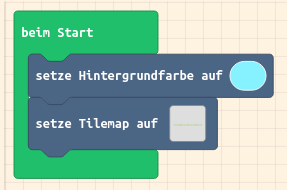
\includegraphics[width=6cm]{game24.png}
  \caption{Erstellen der Map}
  \label{fig:game24}
\end{figure}

\end{frame}

\begin{frame}
 \frametitle{Tilemap bearbeiten}
 
 Ein Klick auf die graue Fläche bringt auch zum Editor der Karte, setzt die Größe auf 50x8 und zeichnet eine Wiese, auf der unsere Spielfigur laufen soll und Lava, über das sie hüpfen muss und ganz zum Schluss eine Zielkachel:
 
\begin{figure}
  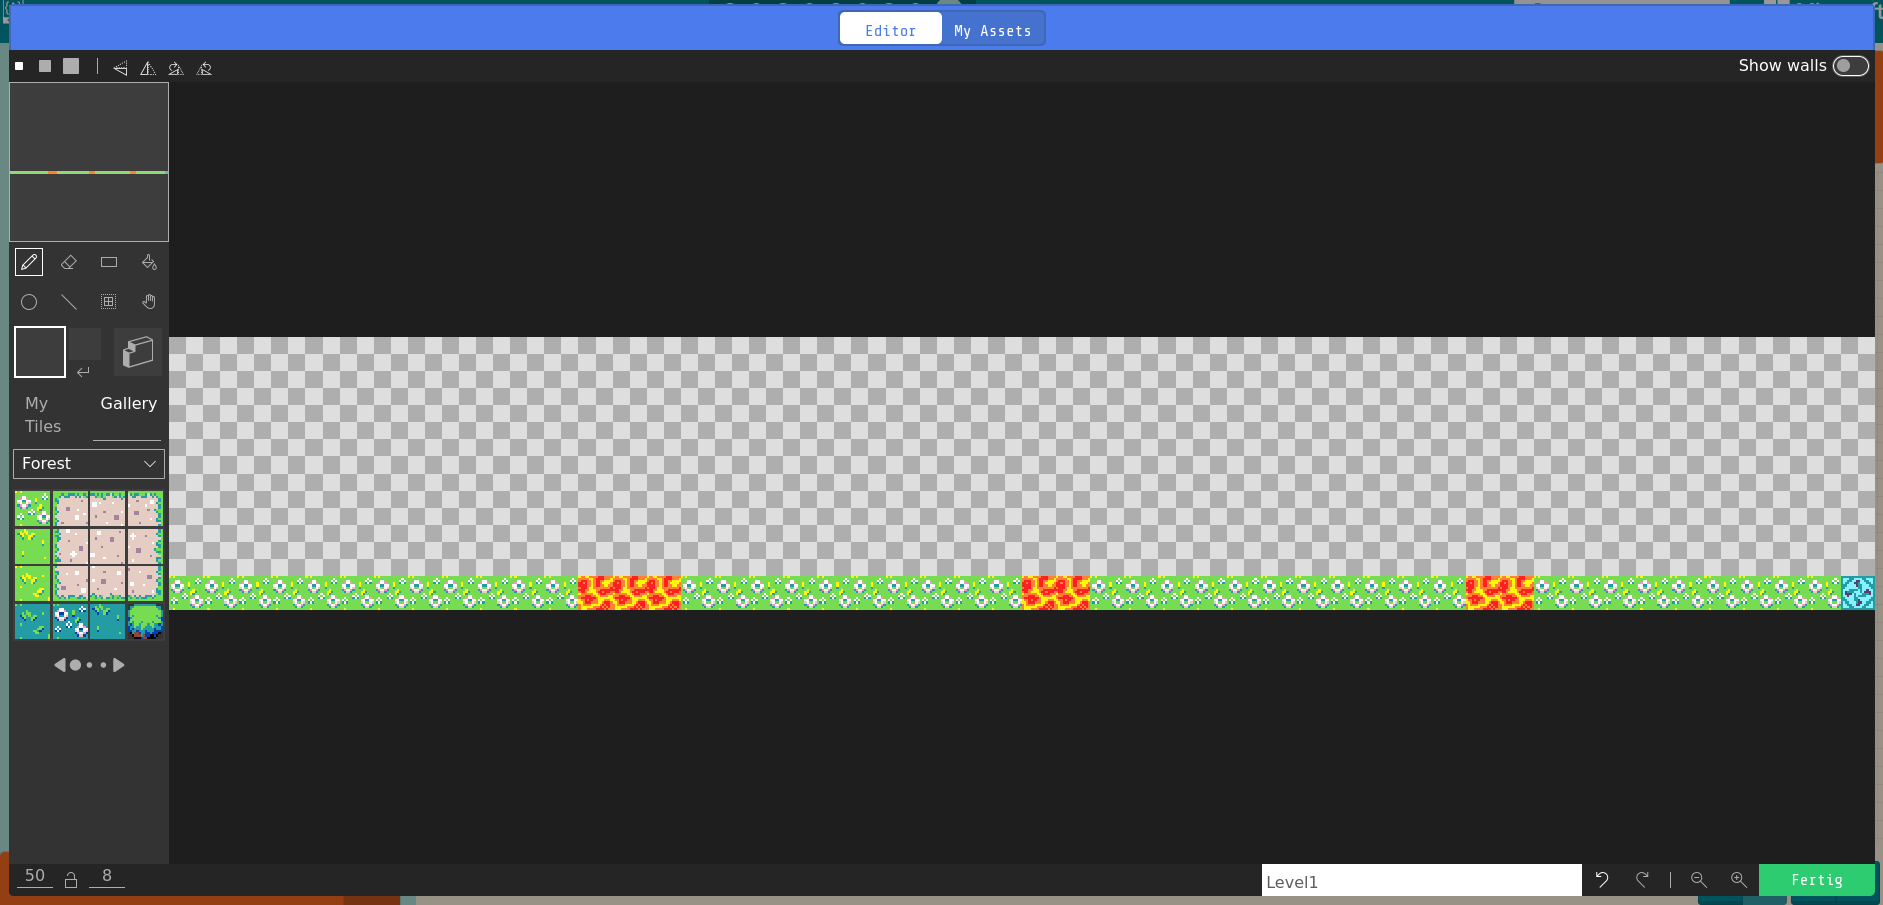
\includegraphics[width=8cm]{game25.png}
  \caption{Bearbeiten der Map}
  \label{fig:game25}
\end{figure}
\end{frame}

\begin{frame}
 \frametitle{Wände einzeichnen}
 
  Mit dem Wandwerkzeug zeichnet Ihr nun Wände – in unserem Fall bei seitlicher Kamera sind das die Plattformen, auf denen die Spielfigur laufen muss. Zeichnet über das Gras, aber nicht über Lava und Zielkachel: 
 
\begin{figure}
  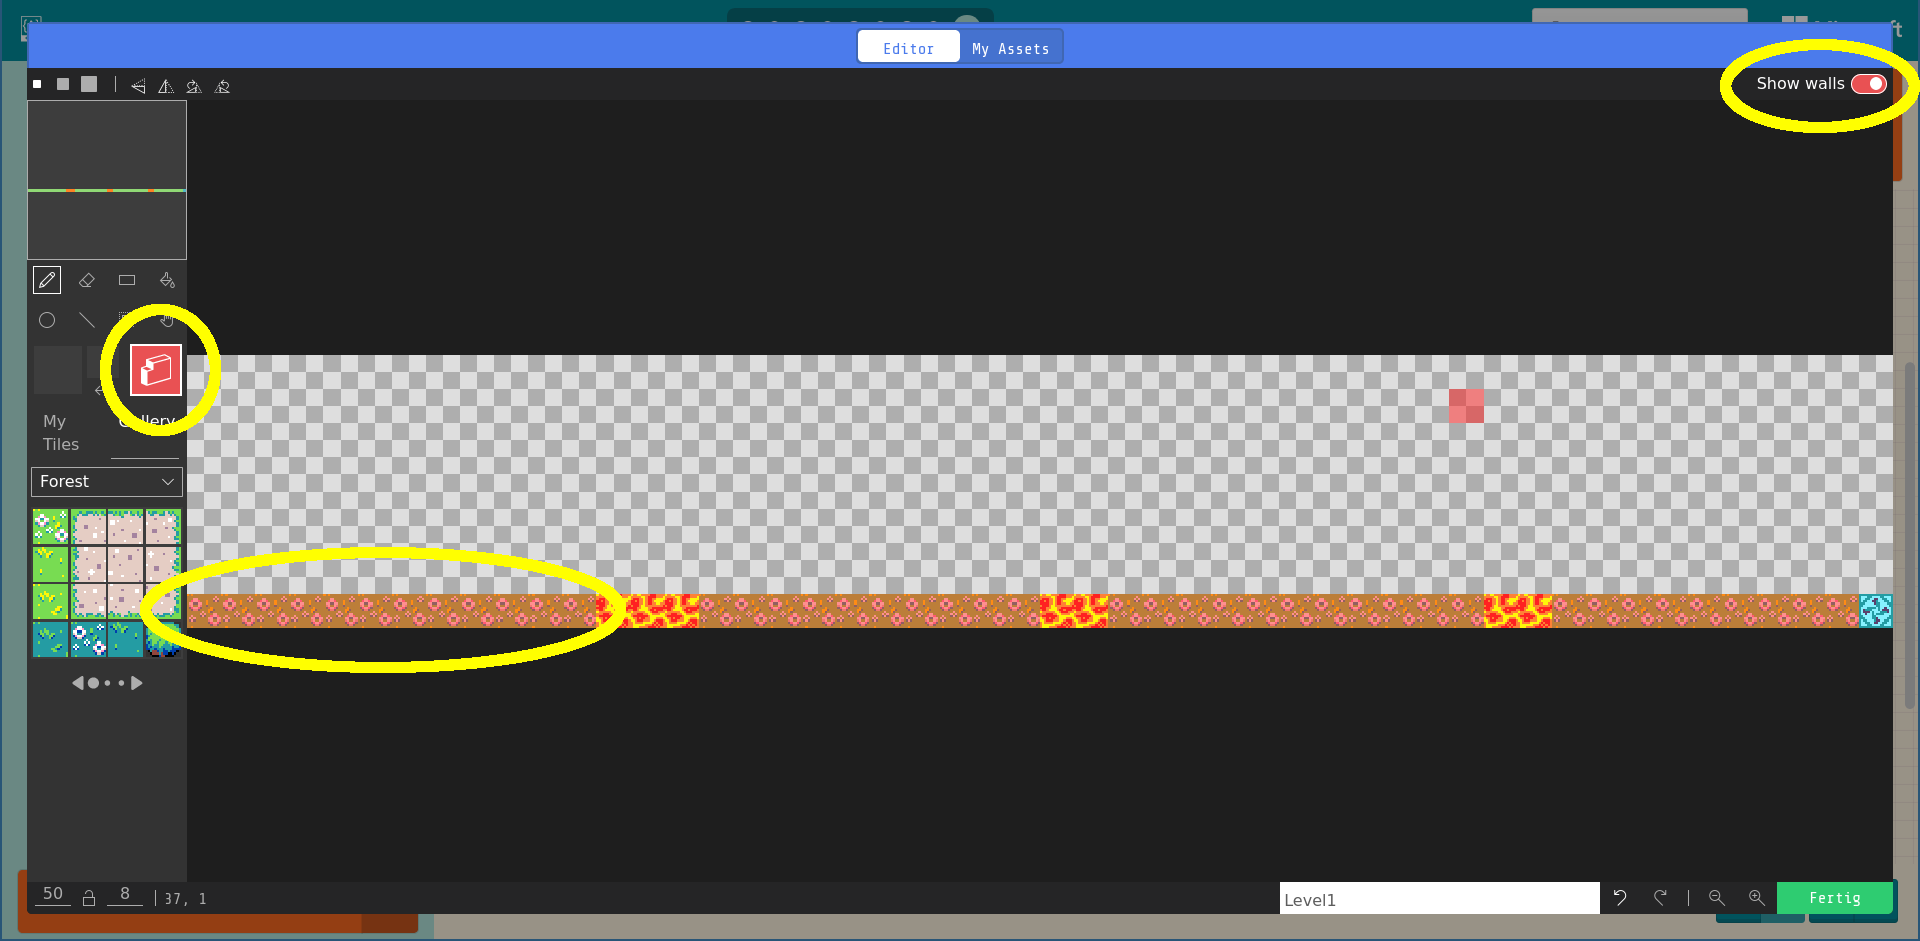
\includegraphics[width=8cm]{game26.png}
  \caption{Wandwerkzeug}
  \label{fig:game26}
\end{figure}
\end{frame}

\begin{frame}
 \frametitle{Spielfigur setzen}
 
 Wählt ein Sprite aus, das als Spielfigur dienen soll und gebt ihm eine X-Geschwindigkeit von ca. 80 Pixeln pro Sekunde mit:
 
\begin{figure}
  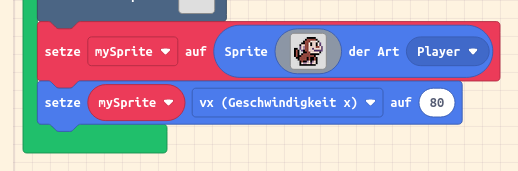
\includegraphics[width=8cm]{game27.png}
  \caption{Affe kommt ins Spiel}
  \label{fig:game27}
\end{figure}
\end{frame}

\begin{frame}
 \frametitle{Gravitation einstellen}
 
 Der Affe schwebt aus dem Bild? Wir sorgen dafür, dass die Kamera der Spielfigur folgt und führen eine Y-Beschleunigung als Gravitation ein. Die sorgt auch dafür, dass der Affe später beim Hüpfen auf den Boden zurückkommt. Je nach Map müsst Ihr die Spielfigur evtl. weiter links positionieren:
 
\begin{figure}
  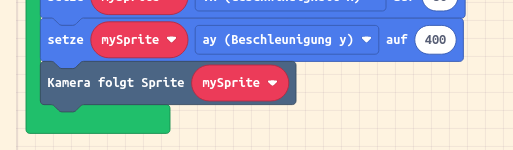
\includegraphics[width=8cm]{game28.png}
  \caption{Gravitation und Kamera}
  \label{fig:game28}
\end{figure}
\end{frame}

\begin{frame}
 \frametitle{Affe hüpf!}
 
Ein Druck auf die A-Taste soll den Affen hüpfen lassen, das erledigt eine negative Y-Geschwindigkeit (zum oberen Bildrand):
 
\begin{figure}
  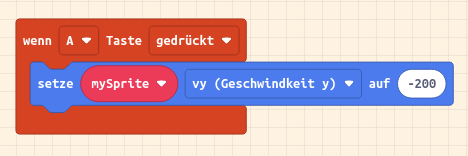
\includegraphics[width=8cm]{game29.png}
  \caption{}
  \label{fig:game29}
\end{figure}
\end{frame}

\begin{frame}
 \frametitle{Schweben verhindern}
 
Wer Dauerfeuer auf A legt, kann komfortabel über alle Hindernisse schweben. Daher soll hüpfen nur möglich sein, wenn die Spielfigur unten auf einer Plattform steht/läuft:
 
\begin{figure}
  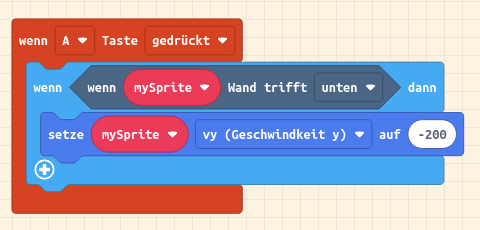
\includegraphics[width=8cm]{game30.png}
  \caption{Wenn-Bedingung verhindert schweben}
  \label{fig:game30}
\end{figure}
\end{frame}

\begin{frame}
 \frametitle{Sieg und Niederlage}
 
 In dieser einfachen Version soll Berühren von Lava das Spiel sofort mit ,,Game Over'' beenden und Erreichen der Zielkachel einen Sieg bedeuten – hierfür gibt es Events für das Berühren von Kacheln:
 
\begin{figure}
  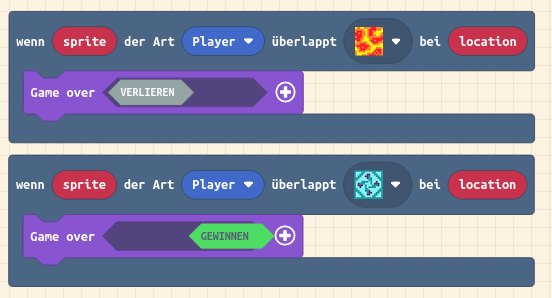
\includegraphics[width=8cm]{game31.png}
  \caption{Kollision mit Kacheln}
  \label{fig:game31}
\end{figure}
\end{frame}

\begin{frame}
 \frametitle{Fertig!}
 
 Zwischenstand nach einer Stunde: Das Jump'n'Run ist so bereits spielbar, aber etwas langweilig:
 
\begin{figure}
  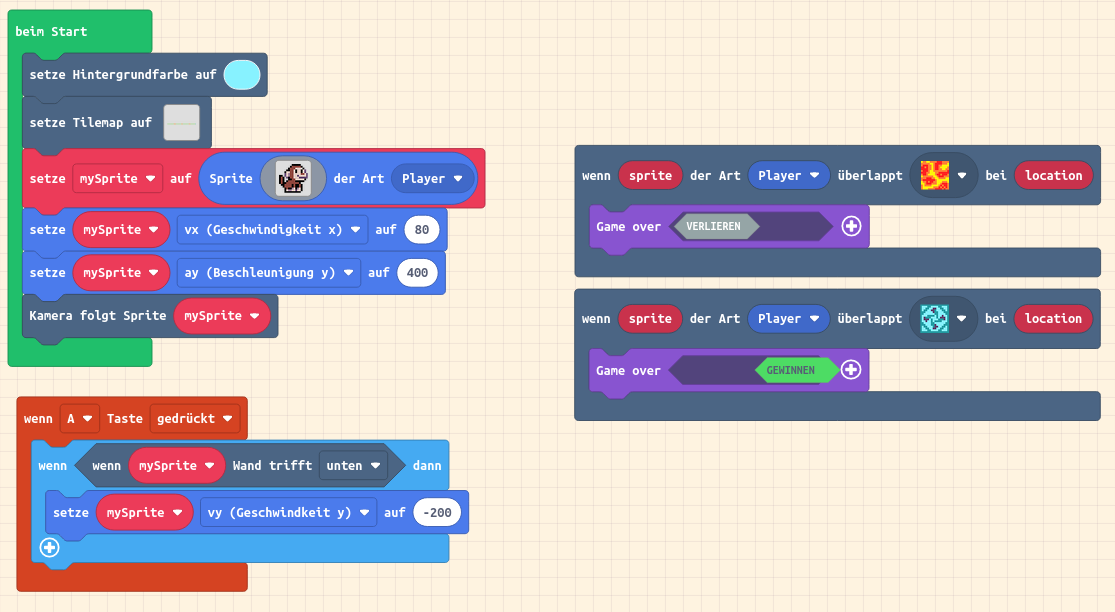
\includegraphics[width=8cm]{game32.png}
  \caption{Zwischenstand}
  \label{fig:game32}
\end{figure}
\end{frame}

\begin{frame}
 \frametitle{Sprite steuern}
 
 Also legen wir die Bewegung des Sprites aufs Steuerkreuz und drehen das Sprite in Bewegungsrichtung (Sprite kopieren und im Editor mit dem Flip-Tool spiegeln):
 
\begin{figure}
  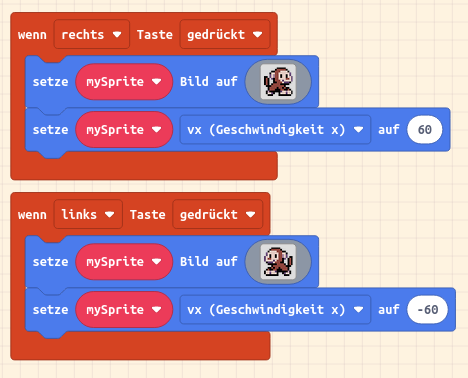
\includegraphics[width=6cm]{game33.png}
  \caption{Sprite mit Richtung}
  \label{fig:game33}
\end{figure}
\end{frame}

\begin{frame}
 \frametitle{Es regnet Haie!}
 
Ihr wolltet eine zusätzliche Gefahr einführen, die von oben kommt. Dafür haben wir Haie bereits mit vY von 200px/s gestartet und beschleunigen sie weiter. Die Position der Haie ist zufällig zwischen 80px links und 80px rechts der Spielfigur:
 
\begin{figure}
  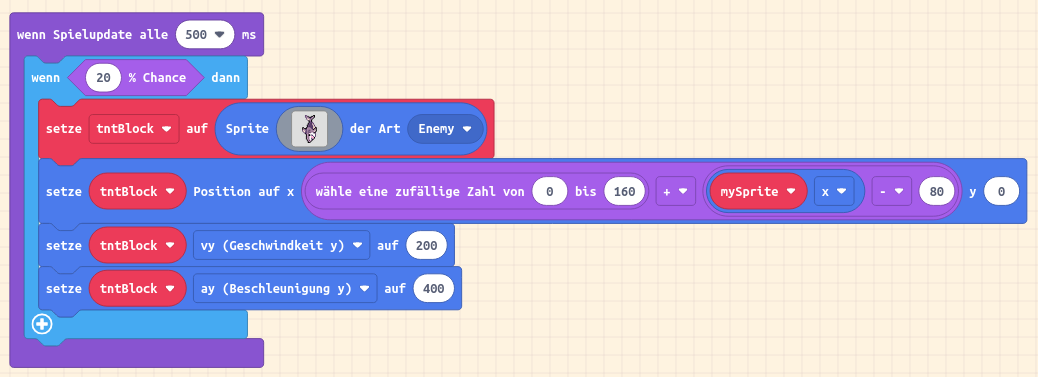
\includegraphics[width=8cm]{game34.png}
  \caption{Achtung, Hairegen!}
  \label{fig:game34}
\end{figure}
\end{frame}

\begin{frame}
 \frametitle{Kollisionserkennung}
 
Natürlich soll der Kontakt mit einem Hai sofortiges ,,Game Over bedeuten'':
 
\begin{figure}
  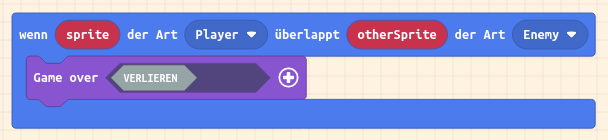
\includegraphics[width=8cm]{game35.png}
  \caption{Game Over!}
  \label{fig:game35}
\end{figure}
\end{frame}

\begin{frame}
 \frametitle{Haie zerschellen}
 
Trifft ein Hai die Plattform, soll er mit einem schönen Effekt zerstört werden, in Lava dagegen einfach reinfallen:
 
\begin{figure}
  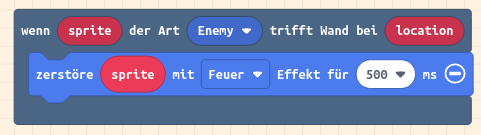
\includegraphics[width=8cm]{game36.png}
  \caption{Hai zerschellt}
  \label{fig:game36}
\end{figure}
\end{frame}

\begin{frame}
 \frametitle{Eine spannendere Tilemap}

Zum Schluss haben wir die Map noch spannender gemacht, mit zusätzlichen Plattformen und Giftpflanzen (Kachel ,,Koralle''), die es zu meiden gilt:
 
\begin{figure}
  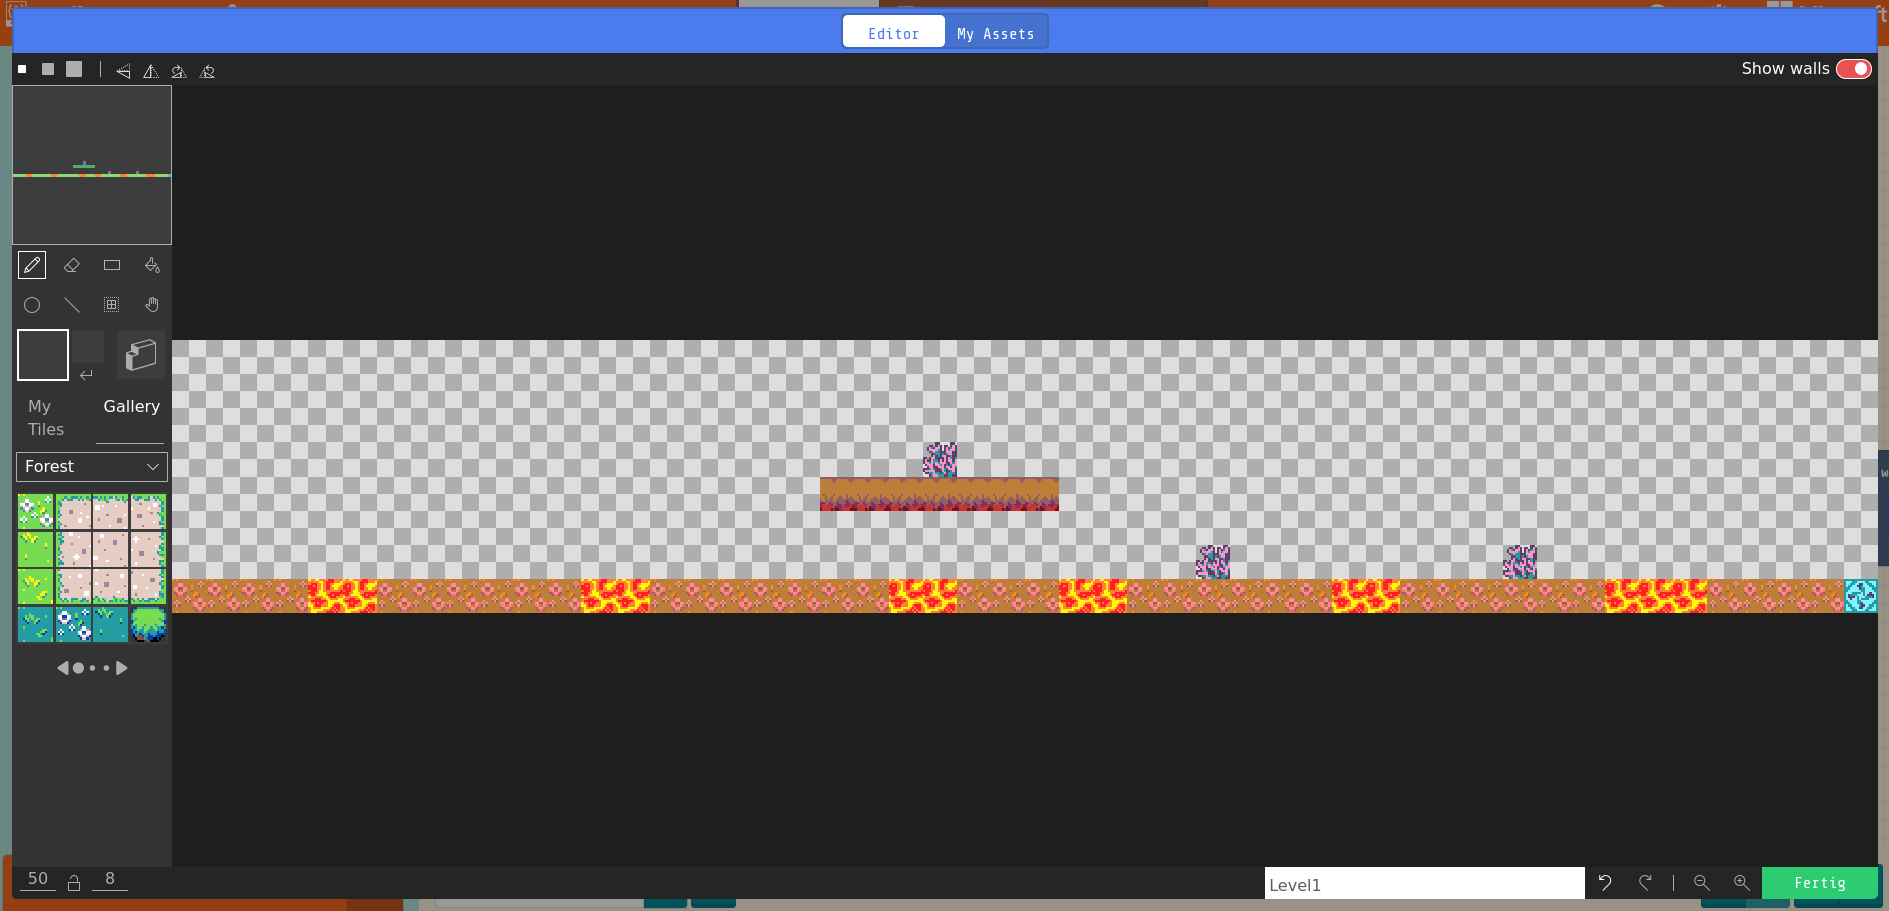
\includegraphics[width=8cm]{game37.png}
  \caption{Map-Editor}
  \label{fig:game37}
\end{figure}
\end{frame}

\begin{frame}
 \frametitle{Download des Musterspiels}

Wie die letzten Termine steht die UF2-Datei in LernSax, alternativ könnt Ihr hier direkt weitermachen:

\href{https://arcade.makecode.com/40668-27213-13741-41735}{https://arcade.makecode.com/40668-27213-13741-41735} 

Wer arbeitet an einer spannenderen Map? Das nächste Mal werden wir Waffen, Werkzeuge und einzusammelnde Münzen einführen…
\end{frame}

\end{document}
